% Part 1: HENRY
\subsection{Objectives}
\begin{frame}{Objectives}
\begin{columns}[c]
    \column{.5\textwidth}
    \begin{block}{Physics}
    \begin{itemize}
        \item Iterative tracking and vertexing may allow high efficiency, high speed, highly parallel algorithms:
        \begin{itemize}
            \item {\bf Use proto-tracks to find primary vertex (PV) candidates}
            \item Use PV candidates to augment more complete tracking
            \item Find more PVs plus secondary vertices
        \end{itemize}
        \item PVs available quickly
    \end{itemize}
    \end{block}
    \column{.5\textwidth}
    \begin{block}{Machine learning}
    \begin{itemize}
        \item Sparse 3D data $\to$ rich 1D dataset
        \item 1D convolutional neural net
        \item Great opportunities to visualize learning process
    \end{itemize}
    \end{block}
    
    \begin{block}{Computation}
    \begin{itemize}
        \item Highly parallelizable
        \item Well suited to GPUs
    \end{itemize}
    \end{block}
\end{columns}


\end{frame}

\subsection{Tracking in the LHCb Upgrade}
\begin{frame}{Tracking in the LHCb Upgrade}
  \begin{columns}[c]
    \column{.5\textwidth}
    \begin{block}{The changes}
      \begin{itemize}
          \item 30 MHz software trigger
          \item 7.6 PVs per event (Poisson distribution)
      \end{itemize}
    \end{block}
    \begin{block}{The problem}
    \begin{itemize}
    	\item Much higher pileup
    	\item Very little time to do the tracking
    	\item Current algorithms too slow
    \end{itemize}
    \end{block}
    \column{.5\textwidth}
      \begin{center}
    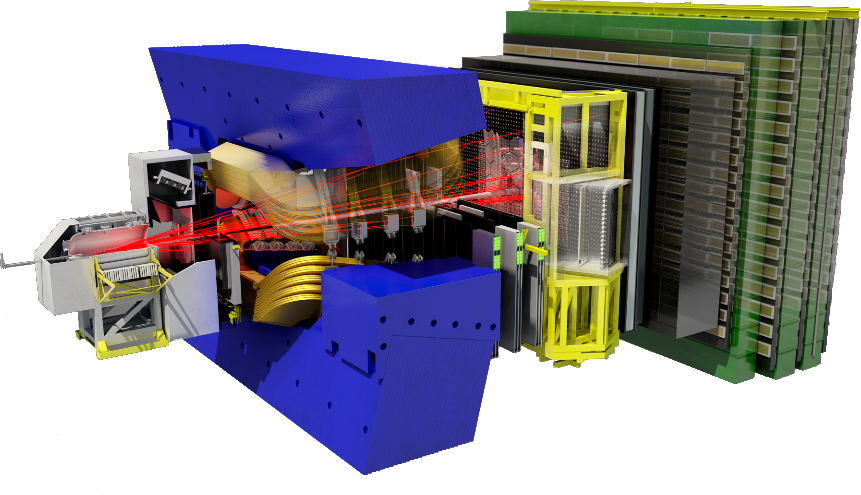
\includegraphics[width=\textwidth, trim=18 0 18 0]{images/LHCbDet.png}
  \end{center}
  \end{columns}
  
  \vspace{1em}
  \begin{center}
    \textbf{We need to rethink our algorithms from the ground up...}
  \end{center}
\end{frame}

\subsection{A Hybrid ML Approach}
\begin{frame}{A Hybrid ML Approach}
\begin{center}
Prototracking $\rightarrow$ Kernel generation $\rightarrow$ CNN to find PVs $\rightarrow$ Informed tracking
\end{center}

\begin{columns}[b]
    \column{.28\textwidth}
    \begin{block}{Prototracking}
    \begin{itemize}
        \item Ultra-simple/fast
        \item Triplets only
        \item Used for kernel only
        \end{itemize}
    \end{block}
    \column{.30\textwidth}
    \begin{block}{Vertexing}
    \begin{itemize}
        \item High efficiency
        \item Low false positive rate
        \item Useful for other reasons
        \end{itemize}
    \end{block}
    \column{.28\textwidth}
    \begin{block}{Tracking}
    \begin{itemize}
        \item Faster (effect TBD)
        \item Uses search windows
        \item Higher efficiency
    \end{itemize}
    \end{block}
\end{columns}
    \begin{block}{Machine learning features (so far)}
        \begin{itemize}
            \item Prototracking converts sparse 3D dataset to feature-rich 1D dataset
            \item Easy and effective visualization due to 1D nature
            \item Can see results with simple unoptimized 2-layer CNN + 1-layer linear
        \end{itemize}
    \end{block}

\vspace{.3em}
\begin{center}
What follows is a proof of principle implementation for finding PVs.
\end{center}
\end{frame}

\subsection{The VELO}
\begin{frame}{The VELO}
  \begin{columns}[c]
    \column{.6\textwidth}
    \begin{block}{Tracks}
      \begin{itemize}
          \item Originate from vertices (not shown)
          \item Hits originate from tracks
          \item We only know the true track in simulation
          \item Nearly straight, but tracks may scatter in material
      \end{itemize}
    \end{block}
    \begin{block}{The VELO}
      \begin{itemize}
          \item A set of 26 planes that detect tracks
          \item Tracks should hit one or more pixels per plane
          \item Sparse 3D dataset (41M pixels)
      \end{itemize}
    \end{block}
    \column{.4\textwidth}
    \centering
    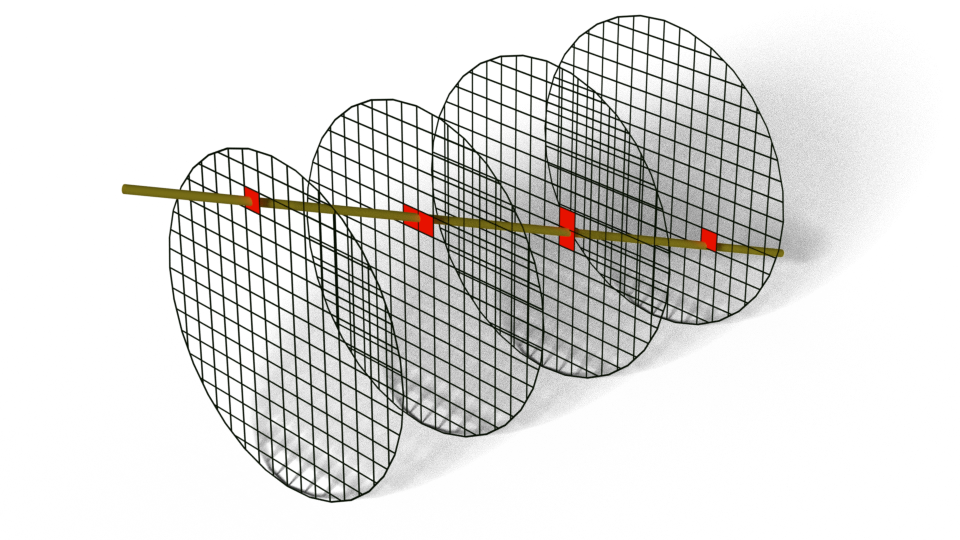
\includegraphics[width=\textwidth, trim=200 0 100 0]{images/Intersections.png}
  \end{columns}
\end{frame}

\subsection{Vertices and Tracks}
\begin{frame}{Vertices and Tracks}
\begin{columns}[c]
    \column{.5\textwidth}
    \begin{block}{Vertices}
      \begin{itemize}
          \item Events contain $\approx 7$ Primary Vertices (PVs)
          \begin{itemize}
            \item A PV should contain 5+ long tracks
          \end{itemize}
          \item Multiple Secondary Vertices (SVs) per event as well
          \begin{itemize}
            \item A SV should contain 2+ tracks
          \end{itemize}
      \end{itemize}
    \end{block}

    \column{.5\textwidth}
    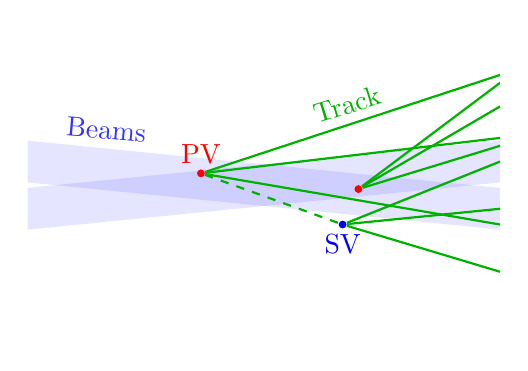
\begin{tikzpicture}
        [beam/.style={line width = 15, opacity=.1, blue, shorten >= -.2cm, shorten <= -.2cm},
        PV/.style={red, circle, fill, inner sep=1pt},
        SV/.style={blue, circle, fill, inner sep=1pt},
        track/.style={green!70!black, thick}]
        
        \clip [use as bounding box] (-3,-2) rectangle (3,2);
        \clip (-3,-2) rectangle (3,2);
        
        \node [blue!80!white, rotate=-5] at (-2, .7) {Beams}; 
        \draw [beam] (-3,.3) -- (3,-.3);
        \draw [beam] (-3,-.3) -- (3,.3);
        
        \node [PV] (A) at (1.2, -.05) {};
        \node [PV] (B) at (-.8, .15) {};
        \node [red, above] at (B) {PV};
        
        \draw [track] (A) -- (3,1.3);
        \draw [track] (A) -- (3,1);
        \draw [track] (A) -- (3,.5);
        
        \draw [track] (B) -- (3,1.4) node [midway, above, rotate=17] {Track};
        \draw [track] (B) -- (3,.6);
        \draw [track] (B) -- (3,-.5);
        \draw [track, dashed] (B) -- (1,-.5);
        
        \node [SV] (C) at (1,-.5) {};
        \node [blue, below] at (C) {SV};
        \draw [track] (C) -- (3, -.3);
        \draw [track] (C) -- (3, .3);
        \draw [track] (C) -- (3, -1.1);
    \end{tikzpicture}
  \end{columns}
  
  \begin{block}{}
  \begin{itemize}
      \item We are developing a way to find PVs and SVs using hit triplets
      \item This will enable an iterative tracking algorithm
  \end{itemize}
  \end{block}
\end{frame}
